\documentclass[tikz,border=2pt]{standalone}
\usepackage{amsmath,amssymb}
\usepackage{xcolor}
\usetikzlibrary{positioning}
\begin{document}
% Extracted from namuenofull.inc; source column: \footnotesize \cite{NU}$_{\rm p{ 165 }}$ II$^*$-IV$^*$-$\alpha$
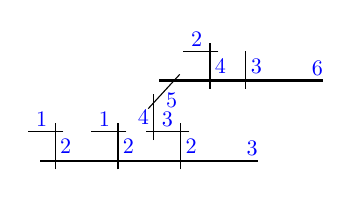
\begin{tikzpicture}[xscale=0.57,yscale=0.62]
\draw[thick,shorten >=2] (4/15,0)--(157/30,0) node[inner sep=2pt,blue,above left,scale=0.8] {3} node[inner sep=2pt,below left,scale=0.8] {};
\draw[shorten <=-3pt, shorten >=-3pt] (3/5,0)--node[inner sep=2pt,scale=0.8,blue,right] {2} (3/5,3/5);
\draw[shorten <=-3pt] (3/5,3/5)--node[inner sep=2pt,scale=0.8,blue,above] {1} (0,3/5);
\draw[shorten <=-3pt, shorten >=-3pt] (2,0)--node[inner sep=2pt,scale=0.8,blue,right] {2} (2,3/5);
\draw[shorten <=-3pt] (2,3/5)--node[inner sep=2pt,scale=0.8,blue,above] {1} (7/5,3/5);
\draw[shorten <=-3pt, shorten >=-3pt] (17/5,0)--node[inner sep=2pt,scale=0.8,blue,right] {2} (17/5,3/5);
\draw[shorten <=-3pt, shorten >=-3pt] (17/5,3/5)--node[inner sep=2pt,scale=0.8,blue,above] {3} (14/5,3/5);
\draw[shorten <=-3pt, shorten >=-3pt] (14/5,3/5)--node[inner sep=2pt,scale=0.8,blue,left] {4} (14/5,6/5);
\draw[shorten <=-3pt, shorten >=-3pt] (14/5,6/5)--node[inner sep=2pt,scale=0.8,blue,below right=-1pt and -1pt] {5} (13/4,33/20);
\draw[thick,shorten >=2] (35/12,33/20)--(401/60,33/20) node[inner sep=2pt,blue,above left,scale=0.8] {6} node[inner sep=2pt,below left,scale=0.8] {};
\draw[shorten <=-3pt, shorten >=-3pt] (81/20,33/20)--node[inner sep=2pt,scale=0.8,blue,right] {4} (81/20,9/4);
\draw[shorten <=-3pt] (81/20,9/4)--node[inner sep=2pt,scale=0.8,blue,above] {2} (69/20,9/4);
\draw[shorten <=-3pt] (97/20,33/20)--node[inner sep=2pt,scale=0.8,blue,right] {3} (97/20,9/4);
\end{tikzpicture}
\end{document}
